
                                                                                                                                                                                                                                                                                                                                                                                                                                                                                                                                                                                                                                                                                                                                                                                                                                                                                                                                                                                                                                                                                                                                                                                                                                                                                                                                                                                                                                                                                                                                                                                                                                                                                                                                                                                                                                                                                                                                                                                                                                                                                                                                                                                                                                                                                                                                                                                                                                                                                                                                                                                                                                                                                                                                                                                                                                                                                                                                                                                                                                                                                                                                                                                                                                                                                                                                                                                                                                                                                                                                                                                                                                                                                                                                                                                                                                                                                                                                                                                                                                                                                                                                                                                                                                                                                                                                                                                                                                                                                                                                                                                                                                                                                                                                                                                                                                                                                                                                                                                                                                                                                                                                                                                                                                                                                                                                                                                                                                                                                                                                                                                                                                                                                                                                                                                                                                                                                                                                                                                                                                                                                                                                                                                                                                                                                                                                                                                                                                                                                                                                                                                                                                                                                                                                                                                                                                                                                                                                                                                             %2multibyte Version: 5.50.0.2890 CodePage: 65001
%\input{tcilatex}
%\input{tcilatex}
%\input{tcilatex}
%\input{tcilatex}


\documentclass[notes=show]{beamer}
%%%%%%%%%%%%%%%%%%%%%%%%%%%%%%%%%%%%%%%%%%%%%%%%%%%%%%%%%%%%%%%%%%%%%%%%%%%%%%%%%%%%%%%%%%%%%%%%%%%%%%%%%%%%%%%%%%%%%%%%%%%%%%%%%%%%%%%%%%%%%%%%%%%%%%%%%%%%%%%%%%%%%%%%%%%%%%%%%%%%%%%%%%%%%%%%%%%%%%%%%%%%%%%%%%%%%%%%%%%%%%%%%%%%%%%%%%%%%%%%%%%%%%%%%%%%
\usepackage{mathpazo}
\usepackage{hyperref}


\usepackage{graphicx}
%\usepackage[spanish]{babel}
\usepackage[latin1]{inputenc}
\usepackage{listings}
\usepackage{amsmath}
\usepackage{amsfonts}
\usepackage{amsxtra}
\usepackage{amstext}
\usepackage{amssymb}
\usepackage{latexsym}
\usepackage{subfigure}
\usepackage{eurosym}
\linespread{1.2}
\usepackage{multimedia}
\usepackage{dsfont} % for \mathds{N}
\usepackage{graphicx}
\usepackage{color,colortbl}
\usepackage{multirow}
\definecolor{clearBlue}{cmyk}{0.15,0.1,0,0.1}
\usepackage{bbm}

%TCIDATA{OutputFilter=LATEX.DLL}
%TCIDATA{Version=5.50.0.2890}
%TCIDATA{Codepage=65001}
%TCIDATA{<META NAME="SaveForMode" CONTENT="1">}
%TCIDATA{BibliographyScheme=Manual}
%TCIDATA{LastRevised=Sunday, April 01, 2012 14:26:41}
%TCIDATA{<META NAME="GraphicsSave" CONTENT="32">}

\newenvironment{stepenumerate}{\begin{enumerate}[<+->]}{\end{enumerate}}
\newenvironment{stepitemize}{\begin{itemize}[<+->]}{\end{itemize} }
\newenvironment{stepenumeratewithalert}{\begin{enumerate}[<+-| alert@+>]}{\end{enumerate}}
\newenvironment{stepitemizewithalert}{\begin{itemize}[<+-| alert@+>]}{\end{itemize} }
\usetheme{Singapore}

%\input{tcilatex}

\begin{document}

\title[Moment Inequalities]{Applications of Moment Inequalities:\\ Ho (2009) \\ + \\ Ho, Ho, and Mortimer (2011)}
\author[MJ Dickstein]{Michael J. Dickstein \\
%EndAName
Stanford University}
\institute{Economics 258}
%\date[3/11/13]{March 11, 2013}
\maketitle

%--------------------------------------------------------------------------------

\section{Inference}

%%%%%%%%%%%%%%%%%%%%%%%%

\begin{frame}
\frametitle{Identified Set}

\begin{itemize}
\item Moment inequalities will generically lead to set identification. Given
a set $S$ of moment inequalities, the identified set is:  
\begin{equation*}
\Theta^{S}=\operatornamewithlimits{argmin}_{\theta}\sum_{s=1}^{S}\Big(\min%
\big\{0,\mathbbm{E}[m_{s}(Y,X,Z;\theta)]\big\}\Big)^{2}
\end{equation*}
\begin{figure}[h!]
\begin{center}
\subfigure{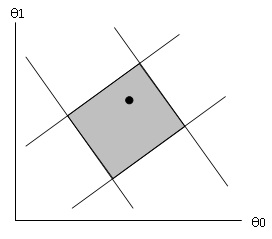
\includegraphics[scale=0.65]{Figure_1.jpg}}  \subfigure{%
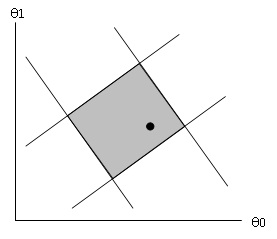
\includegraphics[scale=0.65]{Figure_2.jpg}} 
\end{center}
\end{figure}
\end{itemize}
\end{frame}

%%%%%%%%%%%%%%%%%%%%%%%%

\begin{frame}
\frametitle{Steps for Estimation}

\begin{itemize}
\item Step 1: Estimate the identified set given sample moments. 

\item Step 2: Perform inference on one or more of the following parameters: 

\begin{itemize}
\item Interval contained in the identified set: Pakes, Porter, Ho and Ishii
(2011). 

\item Identified set: Chernozhukov, Hong and Tamer (Econometrica, 2007). 

\item True parameter vector: Andrews and Soares (Econometrica, 2010). 
\end{itemize}
\end{itemize}
\end{frame}

%%%%%%%%%%%%%%%%%%%%%%%%

\begin{frame}[label=estset] 
\frametitle{Estimation of the Identified Set}

\begin{itemize}
\item Estimation is based on the sample analogue of the moment inequalities:
\begin{equation*}
\overline{m}_{n,s}(\theta)=\frac{1}{n}\sum_{i=1}^{n}m_{s}(Y_{i},X_{i},Z_{i};%
\theta)
\end{equation*}
\begin{figure}[h!]
\begin{center}
\subfigure[Case 1]{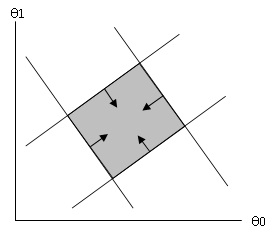
\includegraphics[scale=0.65]{Figure_3.jpg}}  %
\subfigure[Case 2]{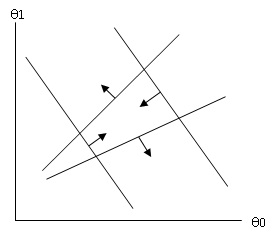
\includegraphics[scale=0.65]{Figure_4.jpg}} 
\end{center}
\end{figure}
\end{itemize}

\end{frame}

%%%%%%%%%%%%%%%%%%%%%%%%

\begin{frame}
\frametitle{Estimation of the identified set}

\begin{itemize}
\item Two possible criterion functions to define the estimated set: 

\begin{itemize}
\item Unweighted criterion function:  
\begin{equation*}
\hat{\Theta}^{S}_{n} = \operatornamewithlimits{argmin}_{\theta}\sum_{s=1}^{S}%
\Big(\min\{0,\overline{m}_{n,s}(\theta)\}\Big)^{2}
\end{equation*}

\item Weighted criterion function:  
\begin{equation*}
\hat{\Theta}^{S}_{n} = \operatornamewithlimits{argmin}_{\theta}\sum_{s=1}^{S}%
\Big(\min\{0,\Big[\frac{\overline{m}_{n,s}(\theta)}{\hat{\sigma}%
^{2}_{n,s}(\theta)}\Big]\}\Big)^{2},
\end{equation*}
with  
\begin{equation*}
\hat{\sigma}^{2}_{n,s}(\theta)=\frac{1}{n}%
\sum_{i=1}^{n}(m_{s}(Y_{i},X_{i},Z_{i};\theta)-\overline{m}%
_{n,s}(\theta))^{2}
\end{equation*}
\end{itemize}

\item The weighting lessens the influence of sample moments that have high
variance (likely to be further away from their population analogues).
\end{itemize}
\end{frame}

%%%%%%%%%%%%%%%%%%%%%%%%

\begin{frame}
\frametitle{Computation of the estimated set}

\begin{itemize}
\item We characterize the set $\hat{\Theta}^{S}_{n}$ by finding its
boundaries along any linear combination of the dimensions of vector $\theta$%
. 

\item If the moment functions $\{\overline{m}_{n,s}(\theta ): s=1,\dots,S\}$
are linear in $\theta$, use linear programming to find the extremum  
\begin{equation}
\begin{split}
& \max_{\theta}\quad f\cdot \theta \\
& \quad \text{s.t.} \\
& \quad \overline{m}_{n,s}(\theta )\geq 0,\text{ for }s=1,...,S.
\label{eq: optvert}
\end{split}%
\end{equation}

\item To find the maximum and minimum of our two-dimensional parameter $%
\theta$, we use:  
\begin{equation*}
f=\{[1,0],[-1,0],[0,1],[0,-1]\}.
\end{equation*}

\item Apply simplex routine in Matlab via \textit{linprog}
\end{itemize}
\end{frame}

%%%%%%%%%%%%%%%%%%%%%%%%

\begin{frame}
\frametitle{Computation of the estimated set}

\begin{itemize}
\item If there is no value of $\theta$ that verifies all the constraints, $%
\hat{\Theta}^{S}_{n}$ will be a singleton. 

\item This singleton is the outcome of a nonlinear optimization problem:  
\begin{equation*}
\hat{\Theta}^{S}_{n} = \operatornamewithlimits{argmin}_{\theta}\sum_{s=1}^{S}%
\Big(\min\{0,\Big[\frac{\overline{m}_{n,s}(\theta)}{\hat{\sigma}%
^{2}_{n,s}(\theta)}\Big]\}\Big)^{2}.
\end{equation*}

\item Use a nonlinear optimization package, like \textit{KNITRO} (in Matlab
via \textit{ktrlink} with license).
\end{itemize}
\end{frame}

%%%%%%%%%%%%%%%%%%%%%%%%

\begin{frame}
\frametitle{Computation of the estimated set: example}

\begin{itemize}
\item Sample moments:  
\begin{eqnarray*}
900-\theta _{0}(-2)-\theta _{1}(60) &\geq &0 \\
-900-\theta _{0}(2)-\theta _{1}(-55) &\geq &0 \\
200-\theta _{0}(1)-\theta _{1}(9) &\leq &0 \\
-200-\theta _{0}(-1)-\theta _{1}(-11) &\leq &0
\end{eqnarray*}
\end{itemize}
\end{frame}

%%%%%%%%%%%%%%%%%%%%%%%%%

\begin{frame}
\frametitle{Computation of the estimated set: example}

\begin{figure}[h!]
\begin{center}
\subfigure{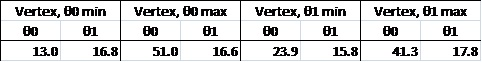
\includegraphics[scale=0.65]{Figure_5.jpg}} \subfigure{%
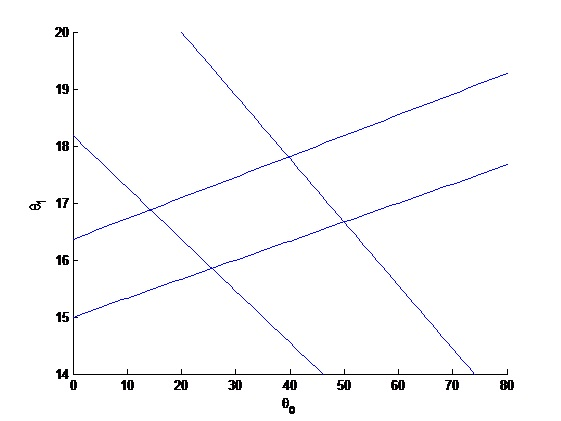
\includegraphics[scale=0.6]{Figure_6.jpg}}
\end{center}
\end{figure}
\end{frame}

%%%%%%%%%%%%%%%%%%%%%%%%%

\begin{frame}
\frametitle{Inference: General Intuition}

\begin{itemize}
\item Consider we want to test the null hypothesis: $H_{0}: \theta=\theta_{0}
$. 

\item We use the following statistic:  
\begin{equation*}
T_{n}(\theta_{0})=\sum_{s=1}^{S}\Big(\min\{0,\Big[\frac{\overline{m}%
_{n,s}(\theta_{0})}{\hat{\sigma}^{2}_{n,s}(\theta_{0})}\Big]\}\Big)^{2}.
\end{equation*}

\item The finite-sample null distribution of $T_{n}(\theta_{0})$ depends on
the degree of \textit{slackness} of the population moments--i.e. how much
greater than 0 is:  
\begin{equation*}
\mathbbm{E}[m_{s}(Y_{i},X_{i},Z_{i};\theta)],\quad\text{for $s=1,\dots,S$}.
\end{equation*}

\end{itemize}
\end{frame}

%%%%%%%%%%%%%%%%%%%%%%%%%

\begin{frame}
\frametitle{Inference: General Intuition}

\begin{itemize}
\item Key: need to infer whether a population moment binds at a particular
value $\theta_{0}$. 

\item Compute slackness factor, $SF_{n,s}(\theta_{0})$ 

\begin{itemize}
\item accounts for whether moment is likely to be binding 

\item moments likely to be nonbinding asymptotically --i.e. $\overline{m}%
_{n,s}(\theta)>>>0$--will have larger slackness factors 
\end{itemize}
\end{itemize}
\end{frame}

%%%%%%%%%%%%%%%%%%%%%%%%%

\begin{frame}
\frametitle{Inference: General Intuition}

\begin{itemize}
\item Three slackness factors proposed in the literature: 

\begin{itemize}
\item Assume that all the $S$ moments are binding at $\theta_{0}$: $%
SF_{I,s}=0$. 

\begin{itemize}
\item yields the most conservative test 
\end{itemize}

\item Moment Selection:  
\begin{equation*}
SF^{MS}_{n,s}(\theta_{0})=\mathbbm{1}\{\sqrt{n}(\frac{\overline{m}%
_{n,s}(\theta_{0})}{\hat{\sigma }_{n,s}(\theta_{0})})\leq\sqrt{2\ln (\ln (n))%
}\}
\end{equation*}

\item Shifted Mean: shift each moment proportionately to how far away from
binding it is in the sample.  
\begin{equation*}
SF^{SM}_{n,s}(\theta_{0})=(\frac{\overline{m}_{n,s}(\theta_{0})}{\hat{\sigma}%
_{n,s}(\theta_{0})})(\frac{1}{\sqrt{2\ln(\ln (n))}})\mathbbm{1}\{\frac{%
\overline{m}_{n,s}(\theta_{0})}{\hat{\sigma}_{n,s}(\theta_{0})}>0\}
\end{equation*}
\end{itemize}
\end{itemize}
\end{frame}

%%%%%%%%%%%%%%%%%%%%%%%%%

\begin{frame}
\frametitle{Inference for an Interval: PPHI (2011)}

\begin{itemize}
\item Objective: build confidence intervals for the vertices of the
estimated set, and use the outer bounds to form a unique confidence
interval. 

\item We need four elements for inference: 

\begin{itemize}
\item Vertices of the estimated set. 

\item Approximation to the asymptotic distribution of all the (weighted)
moments recentered at zero. 

\item Jacobian of the moments. 

\item Slackness factors. 
\end{itemize}
\end{itemize}

\end{frame}

%%%%%%%%%%%%%%%%%%%%%%%%%

\begin{frame}
\frametitle{Inference for an Interval}

\begin{itemize}
\item Approximation to asymptotic distribution of all the recentered
moments. 

\begin{itemize}
\item Draw $r=1,...,R$ times from a multivariate normal with zero mean, and 
covariance equal to the variance of the weighted moments 

\begin{itemize}
\item Take $R$ standard normal draws. 

\item Premultiply each draw by the Cholesky decomposition of the correlation
matrix evaluated at the vertex of interest, $\widehat{\Omega}_{n,S}(\hat{%
\theta})$:  
\begin{equation*}
\widehat{\Omega }_{n,S}(\hat{\theta})=diag(\widehat{\Sigma}_{n,S}(\hat{\theta%
}))^{-\frac{1}{2}}\widehat{\Sigma}_{n,S}(\hat{\theta})diag(\widehat{\Sigma}%
_{n,S}(\hat{\theta}))^{-\frac{1}{2}}.
\end{equation*}

\item Result:  
\begin{equation*}
q_{r}(\hat{\theta})=chol(\widehat{\Omega}_{n,S}(\hat{\theta}))N(0_{S},I_{S}).
\end{equation*}
\end{itemize}
\end{itemize}
\end{itemize}
\end{frame}

%%%%%%%%%%%%%%%%%%%%%%%%%

\begin{frame}
\frametitle{Inference for an Interval}

\begin{itemize}
\item Jacobian of the moments. 

\begin{itemize}
\item Compute the Jacobian of the sample unweighted moments, $\overline{m}%
_{n,s}(\theta)$, and evaluate the result at the vertex of interest: 

\item When the moments are linear in $\theta $, the derivative matrix
multiplied by $\theta $ simply equals the mean of the weighted moments:%
\begin{equation*}
\widehat{\Gamma }_{n,s}(\theta )\ast \theta =\frac{1}{n}\left[
\sum_{i=1}^{n}\frac{\Delta x_{i,s}}{\widehat{\sigma }_{n,s}(\theta )}%
,\sum_{i=1}^{n}\frac{\Delta y_{i,s}}{\widehat{\sigma }_{n,s}(\theta )%
}\right] \ast \binom{\theta _{0}}{\theta _{1}}=\frac{m_{n,s}(\theta )}{%
\widehat{\sigma }_{n,s}(\theta )}
\end{equation*}
\end{itemize}

\item evaluate the weights, $\widehat{\sigma }_{n,s}(\theta )$, at $\theta $
values equal to the relevant vertex.
\end{itemize}
\end{frame}

%%%%%%%%%%%%%%%%%%%%%%%%%

\begin{frame}
\frametitle{Inference for an Interval}

\begin{itemize}
\item Evaluate the slackness factor at the vertex of interest and normalize
by $\sqrt{n}$. 

\begin{itemize}
\item We could use either $SF_{n,s}^{MS}$ or $SF_{n,s}^{SM}$.\newline
The option described in Pakes, Porter, Ho, and Ishii (2011) is Shifted Mean: 
\begin{equation*}
SF_{n,s}^{SM}(\hat{\theta})\sqrt{n}=(\frac{\overline{m}_{n,s}(\hat{\theta})}{%
\hat{\sigma}_{n,s}(\hat{\theta})})(\frac{1}{\sqrt{2\ln (\ln (n))}})%
\mathbbm{1}\{\frac{\overline{m}_{n,s}(\hat{\theta})}{\hat{\sigma}_{n,s}(\hat{%
\theta})}>0\}\sqrt{n}
\end{equation*}
\end{itemize}
\end{itemize}
\end{frame}

%%%%%%%%%%%%%%%%%%%%%%%%%

\begin{frame}
\frametitle{Inference for an Interval}

\begin{itemize}
\item Compute the following linear programing problem for each draw $%
r=1,...,R$ and each vertex $\hat{\theta}$: (total of $2xdxR$ optimizations)  
\begin{equation}
\begin{split}
& \theta _{r}=\max_{\theta }\quad f\cdot \sqrt{n}(\hat{\theta}-\theta ) \\
& \quad \text{s.t.} \\
& \quad \widehat{\Gamma }_{n,S}(\hat{\theta})\sqrt{n}(\hat{\theta}-\theta
)+q_{r}(\hat{\theta})+SF_{n,S}^{SM}(\hat{\theta})\sqrt{n}\geq 0
\end{split}%
\end{equation}

\item As before, to find the maximum and minimum of our
two-dimensional parameter $\theta$, we use:  
\begin{equation*}
f=\{[1,0],[-1,0],[0,1],[0,-1]\}.
\end{equation*}
In equation (2), use the estimated
vertex $\hat{\theta}$ that corresponds to each vector $f$. 

\item We obtain $R$ draws of the asymptotic distribution of each of the
estimated vertices of the estimated set.
\end{itemize}
\end{frame}

%%%%%%%%%%%%%%%%%%%%%%%%%

\begin{frame}
\frametitle{Inference for an Interval}

\begin{itemize}
\item For each pair of vertices corresponding to a given dimension $d$ of $%
\theta$. 

\begin{itemize}
\item For the min vertex, take the $\alpha/2$ quantile of the set of
simulated vertices, $\theta_{r}$, $r=1,\dots,R$. Denote this number:  
\begin{equation*}
\underline{\theta}_{d,\alpha/2}.
\end{equation*}

\item For the max vertex, take the $(1-\alpha/2)$ quantile of the set of
simulated vertices, $\theta_{r}$, $r=1,\dots,R$  
\begin{equation*}
\overline{\theta}_{d,1-\alpha/2}.
\end{equation*}
\end{itemize}

\item The confidence interval for $\theta$ in the dimension $d$ with
significance level $\alpha$ is:  
\begin{equation*}
(\underline{\theta}_{d,\alpha/2},\overline{\theta}_{d,\alpha/2}).
\end{equation*}
\end{itemize}
\end{frame}

%%%%%%%%%%%%%%%%%%%%%%%%%

\begin{frame}
\frametitle{Set/Point Inference: General Intuition}

\begin{itemize}
\item Based on the inversion of an Anderson-Rubin T statistic. 

\item General steps in the algorithm: 

\begin{enumerate}
\item Define $\theta $ grids, $\widehat{\Theta }_{n}^{Grid}$ and $\widehat{%
\Theta }_{n}^{\epsilon }$, where $\widehat{\Theta }_{n}^{\epsilon }\subset 
\widehat{\Theta }_{n}^{Grid}$. 

\item Calculate $T_{r}(\theta )$, at a set of points in either $\widehat{%
\Theta }_{n}^{Grid}$ or $\widehat{\Theta }_{n}^{\epsilon }$ depending on
whether the focus of inference is the identified set or the true value of
the parameter. 

\item Determine a critical value as a quantile of $T_{r}(\theta)$ for $%
r=1,...,R$ 

\item Calculate $T^{obs}(\theta )$ at each $\theta \in \widehat{\Theta }%
_{n}^{Grid}$ with the observed data for all moments. 

\item Define the confidence set as those $\theta$ points where $%
T^{obs}(\theta)$ falls below the critical value. 
\end{enumerate}
\end{itemize}
\end{frame}

%%%%%%%%%%%%%%%%%%%%%%%%%

\begin{frame}
\frametitle{Forming the Grids: $\widehat{\Theta}_{I}^{Grid}$ and
$\widehat{\Theta}_{I}^{\epsilon}$}

$\widehat{\Theta }_{n}^{\epsilon }\subset \widehat{\Theta }_{n}^{Grid}$

\begin{figure}[h!]
\begin{center}
\subfigure{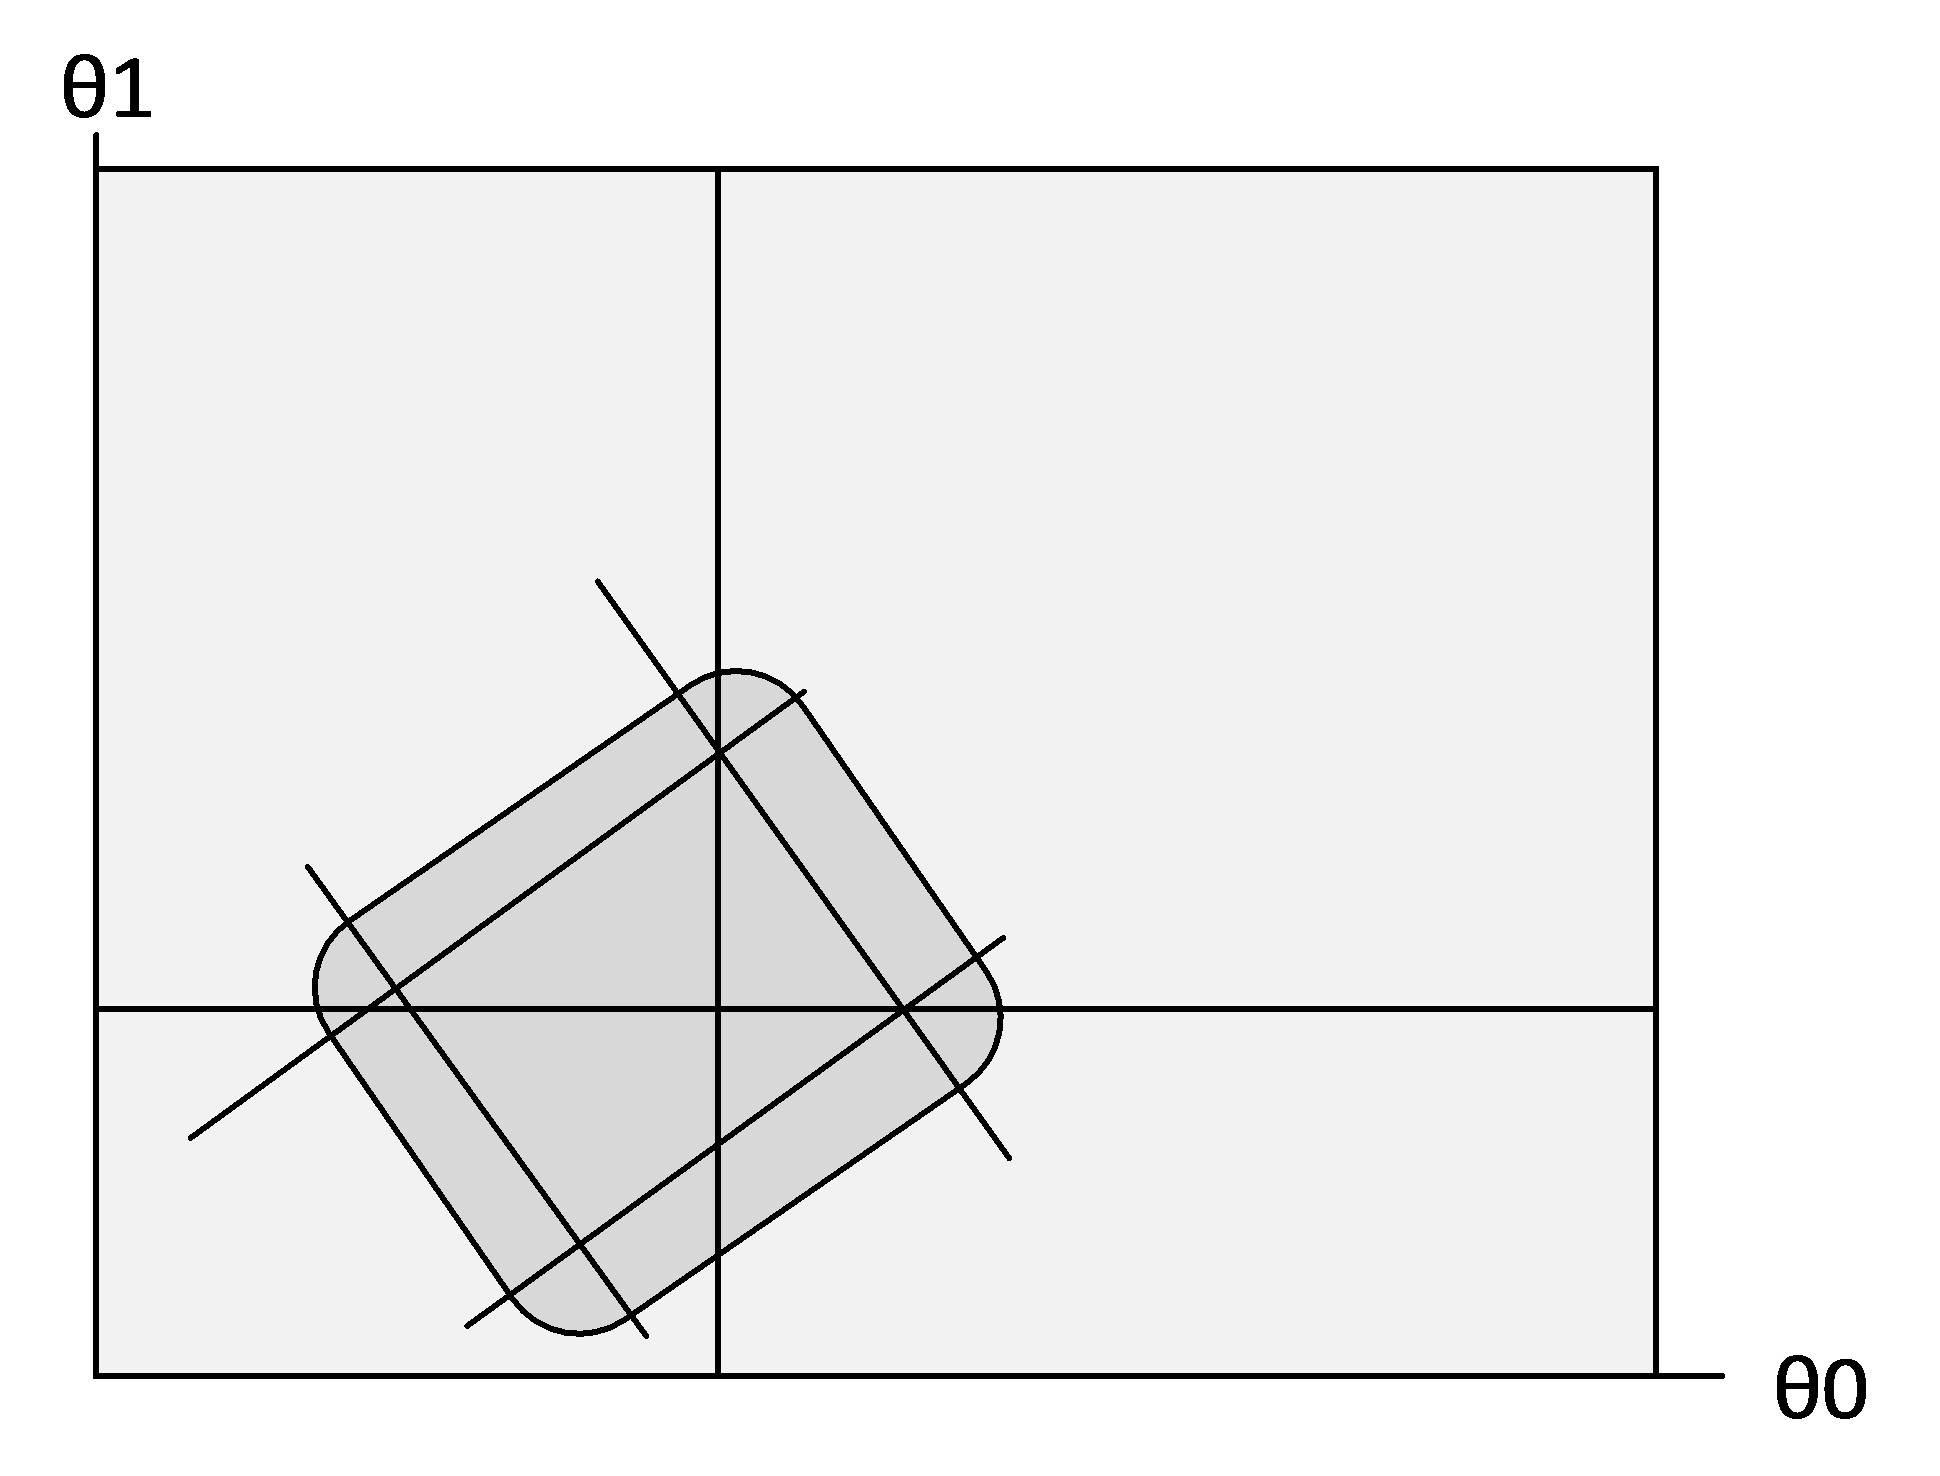
\includegraphics[scale=0.18]{Figure_9.jpg}}
\end{center}
\end{figure}
\end{frame}

%%%%%%%%%%%%%%%%%%%%%%%%%

\begin{frame}
\frametitle{Inference for the Identified Set}
\framesubtitle{Chernozhukov, Hong and Tamer (Econometrica,
2007)}
\begin{itemize}
\item Steps of the procedure: 

\begin{itemize}
\item (1) At $\theta \in \widehat{\Theta }_{n}^{\varepsilon }$, compute R
draws $\{q^{r}(\theta );r=1,\dots ,R\}$ such that: 
\begin{equation*}
q_{r}(\theta )=chol(\widehat{\Omega }_{n,S}(\theta ))N(0_{S},I_{S}),
\end{equation*}%
with 
\begin{equation*}
\widehat{\Omega }_{n,S}(\hat{\theta})=diag(\widehat{\Sigma }_{n,S}(\hat{%
\theta}))^{-\frac{1}{2}}\widehat{\Sigma }_{n,S}(\hat{\theta})diag(\widehat{%
\Sigma }_{n,S}(\hat{\theta}))^{-\frac{1}{2}}.
\end{equation*}%
Note that we are taking draws from the asymptotic distribution of the
normalized recentered moments, evaluated at each point $\theta $. 
\end{itemize}
\end{itemize}
\end{frame}

%%%%%%%%%%%%%%%%%%%%%%%%%

\begin{frame}
\frametitle{Inference for the Identified Set}

\begin{itemize}
\item Steps of the procedure (cont.) 

\begin{itemize}
\item (2) Compute one of the following T-statistic for each value of $\theta 
$ and draw $r$: 
\begin{equation*}
\begin{split}
T_{r}^{N}(\theta )& =\sum_{s=1}^{S}(\min \{0,q_{r,s}(\theta )\})^{2} \\
T_{r}^{MS}(\theta )& =\sum_{s=1}^{S}\{(\min \{0,q_{r,s}(\theta
)\})^{2}\times SF_{n,s}^{MS}(\theta )\} \\
T_{r}^{SM}(\theta )& =\sum_{s=1}^{S}(\min \{0,q_{r,s}(\theta
)+SF_{n,s}^{SM}(\theta )\})^{2}
\end{split}%
\end{equation*}

\item (3) For each draw $r$, take the maximum across $\theta $: 
\begin{equation*}
T_{r}^{\max }=\max_{\theta \in \widehat{\Theta }_{n}^{\varepsilon
}}T_{r}^{k}(\theta ),\quad k=\{N,MS,SM\}.
\end{equation*}
\end{itemize}
\end{itemize}
\end{frame}

%%%%%%%%%%%%%%%%%%%%%%%%%

\begin{frame}
\frametitle{Inference for the Identified Set}

\begin{itemize}
\item Steps of the procedure (cont.) 

\begin{itemize}
\item (4) Compute the critical value $c_{\alpha}$ as the $1-\alpha$ quantile
of the distribution of $\{T^{\max}_{r}; r=1,\dots,R\}$. 

\item (5) Return to the larger grid of theta points, $\widehat{\Theta }%
_{n}^{Grid}$, and calculate $T^{obs}(\theta )$ at each candidate value $%
\theta \in \widehat{\Theta }_{n}^{Grid}$: 
\begin{equation*}
T^{obs}(\theta )=\sum_{s=1}^{S}(\min \{0,\frac{\overline{m}_{n,s}(\theta )}{%
\hat{\sigma}_{n,s}(\theta )}\})^{2}
\end{equation*}

\item (6) Compare $T^{obs}(\theta)$ against $c_{\alpha}$ and accept $\theta$
into the confidence set whenever $T^{obs}(\theta)$ $<$ $c_{\alpha}$. 
\end{itemize}
\end{itemize}
\end{frame}

%%%%%%%%%%%%%%%%%%%%%%%%%

\begin{frame}
\frametitle{Inference for the Identified Set: Example}

\begin{figure}[h!]
\begin{center}
\subfigure{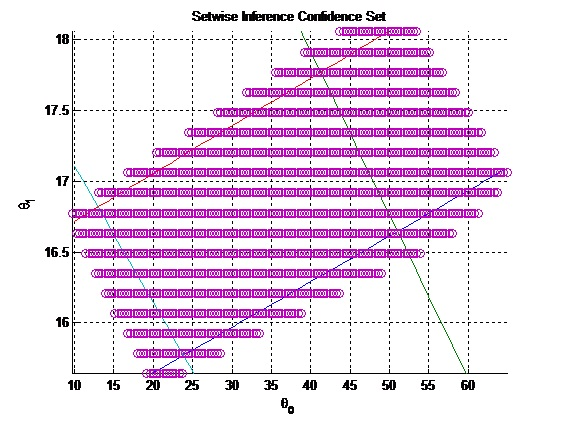
\includegraphics[scale=0.65]{Figure_10.jpg}}
\end{center}
\end{figure}
\end{frame}

%%%%%%%%%%%%%%%%%%%%%%%%%

\begin{frame}
\frametitle{Inference for the True Parameter}
\framesubtitle{Andrews and Soares (2010)}

\begin{itemize}
\item Steps of the procedure: 

\begin{itemize}
\item (1) At every $\theta \in \widehat{\Theta }_{n}^{Grid}$, calculate $%
\{q_{r}(\theta );$ $r=1,\dots ,R\}$: 
\begin{equation*}
q_{r}(\theta )=chol(\widehat{\Omega }_{n,S}(\theta ))N(0_{S},I_{S})
\end{equation*}

\item (2) For each of these $\theta $ and $r$, calculate: $T_{r}(\theta )$, $%
T_{r}^{MS}(\theta )$, or $T_{r}^{SM}(\theta )$. 

\item (3) For each $\theta $, calculate the $(1-\alpha )$ quantile. This the
critical value, $c(\alpha ,\theta )$. 

\item (4) Calculate $T^{obs}(\theta )$ at each candidate value $\theta \in 
\widehat{\Theta }_{n}^{Grid}$. 

\item (5) Compare $T^{obs}(\theta )$ against $c(\alpha ,\theta )$ and accept 
$\theta $ into the confidence set whenever $T^{obs}(\theta )$ $<$ $c(\alpha
,\theta )$. 
\end{itemize}
\end{itemize}
\end{frame}

%%%%%%%%%%%%%%%%%%%%%%%%%

\begin{frame}
\frametitle{Comparison of Inference Procedures}

\begin{figure}[h!]
\begin{center}
\subfigure{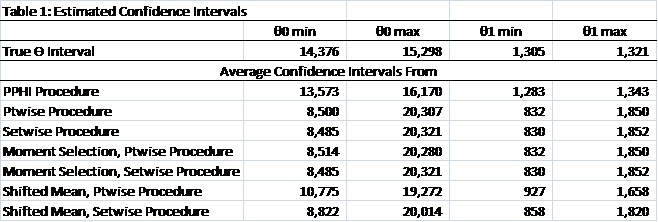
\includegraphics[scale=0.65]{Figure_16.jpg}}
\end{center}
\end{figure}
\end{frame}


%--------------------------------------------------------------------------------
\section{Ho 2009}
%--------------------------------------------------------------------------------

\begin{frame}
\frametitle{Ho 2009}

\begin{itemize}
	\item Theory testing
	\item Measurement
	\item Methodology
\end{itemize}
\end{frame}

%--------------------------------------------------------------------------------

\begin{frame}
\frametitle{Ho 2009}

\begin{itemize}
	\item Theory testing
         \begin{itemize}
	\item Can a bargaining model explain the hospital-insurance plan contracting process, rationalizing the observed network of hospital-plan relationships? 	\end{itemize}
	\item Measurement
	\begin{itemize}
	\item What characteristics of hospitals and plans explain the level of surplus hospitals can extract from the relationship?
	\item What is the effect of capacity constraints on producer welfare?  Might the level of capacity be a relevant choice variable for a profit-maximizing firm?
	\end{itemize}
\end{itemize}
\end{frame}

%--------------------------------------------------------------------------------

\begin{frame}
\frametitle{Ho 2009}

\begin{itemize}
	\item Methodology
	\begin{itemize}
	\item What assumptions are needed on behavior to develop a moment inequality estimator for static contracting problems?
	\item What can information on ex-post network formation reveal about private negotiated prices?
	\end{itemize}
\end{itemize}
\end{frame}

%--------------------------------------------------------------------------------

\begin{frame}
\frametitle{Ho 2009}

Main Idea
\begin{itemize}
	\item Model demand for hospitals and health plans, accounting for the hospital network of each plan in the consumer`s plan choice
	\item Model the supply side negotiation between hospitals and plans in forming equilibrium networks, which determines the division of profits
        \item To increase their share of the surplus from contracting, hospitals have incentives to:
         \begin{itemize}
	\item Invest in quality to attract more patients, lower costs
	\item Merge with other providers, to improve bargaining position
	\item Under-invest in capacity
	\end{itemize}
\end{itemize}
\end{frame}

%--------------------------------------------------------------------------------

\begin{frame}
\frametitle{Ho 2009}

Main Idea
\begin{itemize}
\item Findings
\begin{itemize}
\item ``Star`` hospitals capture \$6700 more per patient than other providers, on costs of \$11,000
\item Hospitals with capacity constraints have markups of \$6900 per patient more than those without constraints
\item System hospitals have \$180,000/month greater profits than other providers
\end{itemize}
\end{itemize}
\end{frame}

%--------------------------------------------------------------------------------

\begin{frame}
\frametitle{Ho 2009}

Data
\begin{itemize}
\item Insurer plan data cover all managed care insurers in 43 major markets across the US for Q3, Q4 of 2002 (cross-section)
\begin{itemize}
\item Premiums earned, number of enrollees, tax status of each carrier
\item Data on clinical performance and patient satisfaction with health plans
\end{itemize}
\item Hospital data from Medstat from private insurers; includes encounter-level data on hospital admissions during 2 year period.
\begin{itemize}
\item Patient`s diagnosis and characteristics, identity of hospital, type of plan
\item Hospital characteristics from AHA
\end{itemize}
\item Data on network of hospitals for every HMO/POS plan in every market considered in March/April 2003

\end{itemize}
\end{frame}

%--------------------------------------------------------------------------------
\begin{frame}
\frametitle{Ho 2009}

Model: Stages
\begin{itemize}
\item 0. Plans choose quality and products; Hospitals choose capacity, location, product mix, system mergers.
\item 1. Hospitals make simultaneous take-it-or-leave-it price offers to all plans in the market
\item 2. Plans choose whether to accept these offers, forming their hospital network
\item 3. Plans set premiums to maximize profits after a change in networks
\item 4. Consumers and employers jointly choose plans
\item 5. Sick consumers visit hospitals; plans pay hospitals per service provided.
\end{itemize}
\end{frame}
%--------------------------------------------------------------------------------
\begin{frame}
\frametitle{Ho 2009}

Model: Hospital Demand
\[
u_{i,h,l}=\eta _{h}+x_{h}\alpha +x_{h}\nu _{i,l}\beta +\varepsilon _{i,h,l}
\]

\begin{itemize}
\item individual i, hospital h, diagnosis l
\item $x_{h}$ observed hospital characteristics
\item $\nu_{i,l}$ observed characteristics of consumers
\item Estimate via ML, using Medstat data
\begin{itemize}
\item Medstat doesn't have hospital networks for managed care enrollees; use only data on indemnity and PPO enrollees whose choice set is unrestricted
\item Assume: indemnity/PPO enrollees have same preferences over hospitals as managed care enrollees (vertical preferences)
\end{itemize}
\end{itemize}

\end{frame}

%--------------------------------------------------------------------------------
\begin{frame}
\frametitle{Ho 2009}

Model: Health Plan Demand
\[
\widetilde{u}_{ijm}=\xi _{jm}+z_{jm}\lambda +\gamma _{1}EU_{ijm}+\gamma _{2}%
\frac{prem_{j,m}}{y_{i}}+\omega _{ijm}
\]

\begin{itemize}
\item individual i, plan j, market m
\item $(z_{jm},\xi_{jm})$ observed and unobserved plan characteristics
\item outside option = choosing to be uninsured; indemnity/PPO is separate choice in each mkt
\item IV for premium
\begin{itemize}
\item plan char, avg hourly hospital wage, avg weekly nurse wage
\item exclusion restriction: health plan costs correlated with premiums but not with unobs plan quality
\end{itemize}
\item Find: consumers value EU from network in plan choice
\end{itemize}

\end{frame}

%--------------------------------------------------------------------------------
\begin{frame}
\frametitle{Ho 2009}

Model: Producer surplus generated by network
\[
S_{j,m}(H_{j},H_{-j})=\sum%
\limits_{i}(n_{i}s_{ijm}(H_{j},H_{-j})[prem_{j,m}-p_{i}\sum \limits_{h\in
H_{j}}s_{i,h}(H_{j})\text{cost}_{h}])
\]

\begin{itemize}
\item The shares $s_{ijm}(H_{j},H_{-j})$ are plan j`s predicted shares of type i people when networks $(H_{j},H_{-j})$ offered (flow of consumers to plans after network changes)
\item $s_{i,h}(H_{j})$ hospitals h`s predicted share of type i people (flow of consumers to hospitals after network change)

\end{itemize}

\end{frame}

%--------------------------------------------------------------------------------
\begin{frame}
\frametitle{Ho 2009}

Model: Producer surplus generated by network
\[
S_{j,m}(H_{j},H_{-j})=\sum%
\limits_{i}(n_{i}s_{i,j,m}(H_{j},H_{-j})[prem_{j,m}-p_{i}\sum \limits_{h\in
H_{j}}s_{i,h}(H_{j})\text{cost}_{h}])
\]

\begin{itemize}
\item Premiums adjust in response to changes in hospital network
\begin{itemize}
\item (1) Estimate supply model assuming fixed premiums
\item (2) Allow all plans to simultaneously adjust their premiums to max profits
\item Comment: with panel data, could push further
\end{itemize}
\item No non-hospital variable costs
\item Adjusts for capacity constraints at 85\% level

\end{itemize}

\end{frame}

%--------------------------------------------------------------------------------
\begin{frame}
\frametitle{Ho 2009}

Model: Negotiation
\begin{itemize}
\item All hospitals make TIOLI offers of \{contract,null offer\}
\item All plans simultaneously respond
\item Offers are private info; plans have passive beliefs (if plan gets an alternative offer from h, doesn't change plan's beliefs about offers h makes to its competitors)

\[
\pi _{j,m}^{P} =S_{j,m}(H_{j},H_{-j})-c_{j,m}^{Hosp}(H_{j},H_{-j},X,\theta
)-c_{j,m}^{nonhosp}(H_{j},H_{-j},X,\theta )
\]
\begin{eqnarray*}
\pi _{j,m}^{P,o}(.) &=&\pi _{j,m}^{P}+\mu _{j,H_{j}} \\
E[\pi _{j,m}^{P}(H_{j},H_{-j},X,\theta )|Ij,m] &=&\pi
_{j,m}^{P}(H_{j},H_{-j},X,\theta )-\varphi _{j,H_{j}}
\end{eqnarray*}

\end{itemize}

\end{frame}

%--------------------------------------------------------------------------------
\begin{frame}
\frametitle{Ho 2009}

Model: Negotiation
\begin{itemize}
\item Key assumption: plan j`s expected profits from $H_{j}$ $>$ expected profits from alternative network formed by reversing contract with h
\[
E[\pi _{j,m}^{P,o}(H_{j},H_{-j},X,\theta )-\pi
_{j,m}^{P,o}(H_{j}^{h},H_{-j},X,\theta )|Z_{j,m}]\geq 0
\]
\item form unconditional moments using positive-valued function of $Z_{j,m}$
\begin{itemize}
\item must be known to firms when they make their choice
\item use char in fixed cost and markup terms other than cost/admission
\item use indicators for some plan and market characteristics
\end{itemize}

\end{itemize}

\end{frame}

%--------------------------------------------------------------------------------
\begin{frame}
\frametitle{Ho 2009}

Model: Negotiation
\begin{itemize}
\item Choose counterfactuals of reversing a single contract.
\item Plans may respond by changing its response to other hospital`s offers (passive beliefs rules out the following: plan responds to changes in h`s offer by assuming other plans have different offers and therefore change their own networks)
\item Two possible routes
\end{itemize}

\end{frame}

%--------------------------------------------------------------------------------
\begin{frame}
\frametitle{Ho 2009}

Model: Negotiation
\begin{itemize}
\item Two possible routes
\begin{itemize}
\item Assume hospital can make an alternative offer to j that will prompt j to drop h from its network and not change its contract with other hospitals
\item Allow plan to adjust its decisions wrt all other hospitals
\begin{itemize}
\item find min of hospital h`s profits from all possible choices plan j can make in response to the deviation (given its other contracts and networks of other plans)
\item form inequality with difference between realized profit and minimized counterfactual profit
\end{itemize}

\end{itemize}
\end{itemize}

\end{frame}

%--------------------------------------------------------------------------------
\begin{frame}
\frametitle{Ho 2009}

Results
\begin{itemize}
\item Estimate of $\theta$ for every specification is a singleton; could not satisfy all inequality constraints.  Why?
\begin{itemize}
\item random disturbances
\item no. of moments used
\item no structural error (some component of profit function not observed by econometrician but used by the agent, that varies at p,h level)
\end{itemize}
\item Comment
\begin{itemize}
\item Inference for moment inequalities that find a set more complicated
\item Counterfactuals in the case of set identification?
\end{itemize}
\end{itemize}
\end{frame}

%--------------------------------------------------------------------------------
\begin{frame}
\frametitle{Ho 2009}

Results: Substantive findings
\begin{itemize}
\item Hospitals in systems take a larger fraction of surplus, penalize plans that do not contract with all members
\item Star hospitals capture high mark-ups
\item Hospitals with higher costs/pt receive lower markups/pt
\end{itemize}
\end{frame}

%--------------------------------------------------------------------------------

\section{Ho, Ho, and Mortimer (2011)}

%--------------------------------------------------------------------------------

\begin{frame}
\frametitle{Goals of the Paper}

\begin{itemize}
\item Theory Testing

\begin{itemize}
\item What are the profit consequences for the manufacturer from offering
retailers full-line forcing contracts?

\item Does it reduce consumer choice or lead to higher prices?
\end{itemize}

\item Measurement

\begin{itemize}
\item Quantify how consumer demand, retailer revenues and costs, and
distributor revenues change when adding/removing FLF from contract mix.
\end{itemize}

\item Methodology

\begin{itemize}

\item \textquotedblleft Role model\textquotedblright \ of bundling analysis:
combine detailed demand side estimation of substitution with supply side
model of firm's costs from adding inventory.
\end{itemize}
\end{itemize}
\end{frame}

%--------------------------------------------------------------------------------

\begin{frame}
\frametitle{Setting}

Innovation in recording rental transactions led to contract innovation:

\begin{itemize}
\item Linear pricing -- \$65-70 upfront fee per tape

\item Revenue sharing - \$8 upfront + 55\% of rental revenue per tape

\begin{itemize}
\item Have min and max quantity restrictions
\end{itemize}

\item FLF -- rental store purchases all titles of distributor

\begin{itemize}
\item Terms like RS, but lower up-front fee (\$3.60) and lower rev share
(retailers keep 59\%)
\end{itemize}

\item Sell-through priced (STP) titles

\end{itemize}
\end{frame}

%--------------------------------------------------------------------------------

\begin{frame}
\frametitle{Setting}

Selection on contract type?

\begin{itemize}
\item What type of movies should retailer choose to accept under each
contract type? (Mortimer (2008))

\begin{itemize}
\item LP for high volume videos/new releases?

\item RS for niche films? RS usually have higher minimum quantity
restrictions than the avg \# of tapes bought under LP contracts.
\end{itemize}

\end{itemize}
\end{frame}

%--------------------------------------------------------------------------------

\begin{frame}
\frametitle{Setting}

How does inventory choice affect retailer profits?

\begin{itemize}
\item Can increase retailer profits by attracting new consumers to store.
(included in costs of holding inventory)

\item High inventory may lead to high initial demand (consumers see more
tapes on shelf); can reduce later month sales (included in costs of holding
inventory)

\item Sales of substitute products fall with higher inventory on focal
product (see demand model)
\end{itemize}
\end{frame}

%--------------------------------------------------------------------------------

\begin{frame}
\frametitle{Model}

Retailer portfolio choice problem

\begin{itemize}
\item Moment inequalities to bound the value of holding inventory (do not
model complicated retailer equilibrium strategies)

\item Intuition:

\begin{itemize}
\item on average, stores' profits from the observed portfolio of
titles and choices of inventory must exceed profits from alternative
portfolios/inventory

\item Dropping a title gives you upper bound to costs of holding inventory

\item Adding tapes (say, 10\%) provides lower bound on value of holding
inventory.
\end{itemize}

\end{itemize}
\end{frame}

%--------------------------------------------------------------------------------
\begin{frame}
\frametitle{Model}

Retailer portfolio choice problem (continued)

Procedure

\begin{itemize}
\item Calculate share of title at store m at time t using demand estimates.

\item Determine total returns to the store under its inventory constraints
(determined by the contracts it entered).

\item Subtract off payments to distributor and the costs of holding a tape
to find profits.
\end{itemize}
\end{frame}

%--------------------------------------------------------------------------------

\begin{frame}
\frametitle{Model}

Inequalities%
\[
E[\pi _{m}^{obs}(.)|I_{m}] \geq E[\pi _{m}^{altj^{\prime }}(.)|I_{m}] 
\]
\[
\pi _{m}^{obs} =\sum_{s}\sum_{j\in J_{s}}(r_{jm}^{obs}(.)-C(.)\widetilde{c}_{jm})+\eta _{m}+\rho (\widetilde{c}_{ms},k_{ms})+\varepsilon _{ms}
\]

\begin{itemize}
\item Assume $\eta _{m}$, $\rho (\widetilde{c}_{ms},k_{ms})$ difference out

\item Have instruments, $Z_{ms^{\prime }}\subset I_{m}$

\item $E[\varepsilon _{ms}|Z_{ms^{\prime }}]=0$

\item Use as IV's \{constant; indicators for size of store\}

\item Rules out error term that differs by contract type and that are
structural--that is, choice of contract depends on error.

\begin{itemize}
\item STRONG - claim is that specification of inventory holding value
captures all elements in $I_{m}$
\end{itemize}
\end{itemize}
\end{frame}

%--------------------------------------------------------------------------------

\end{document}
